\documentclass[oneside, 12pt]{article}

\newcommand{\source}[1]{\textbf{Source:} {#1} }

\usepackage{indentfirst}
\usepackage{listings}
\usepackage{graphicx}
\usepackage{float}
\usepackage{color}
\usepackage{amsmath}
\usepackage[utf8]{inputenc}
\usepackage[english]{babel}
\usepackage[backend=bibtex]{biblatex}
\usepackage{color}
\usepackage{appendix}

\addbibresource{ref.bib}

\definecolor{pblue}{rgb}{0.13,0.13,1}
\definecolor{pgreen}{rgb}{0,0.5,0}
\definecolor{pred}{rgb}{0.9,0,0}
\definecolor{pgrey}{rgb}{0.46,0.45,0.48}

\usepackage{listings}
\lstset{language=Java,
  showspaces=false,
  showtabs=false,
  breaklines=true,
  showstringspaces=false,
  breakatwhitespace=true,
  commentstyle=\color{pgreen},
  keywordstyle=\color{pblue},
  stringstyle=\color{pred},
  basicstyle=\ttfamily,
  moredelim=[il][\textcolor{pgrey}]{\$\$},
  moredelim=[is][\textcolor{pgrey}]{\%\%}{\%\%}
}

\begin{document}
\title{Java 8 Parallel Streams}
\author{Ethan Williams}
\date{\today}
\maketitle

\tableofcontents

\pagebreak

\setcounter{section}{-1}
\section{Prerequisites}

\subsection{Technical}
This document was written for Java developers who have an interest in using concurrency in streams, and assumes knowledge of serial streams and lambda expressions. Developers in other languages with similar mechanisms such as C\# with \verb|Linq| may also find the topics useful with the understanding that syntax, implementation, and functionality will differ.

Additionally, functional knowledge of \verb|java.util.concurrent| and the \verb|Consumer| interface will help in gaining a more practical knowledge but is not required.

\subsection{Vocabulary Clarification} \label{language}
Some of the vocabulary in the paper may be unfamiliar to those with a knowledge of streams and are defined/clarified below:
\begin{itemize}
\item A stream is composed of 3 parts: 
	\begin{itemize}
	\item the \verb|Collection| the stream is built on is the \textit{source}
	\item \textit{intermediate operations} such as \verb|map()| transforms but doesn't serialize the stream (see below for serialization definition) 
	\item \textit{terminal operations} like \verb|toArray()| serialize the stream
	\end{itemize}
\item A stream instantiated with the \verb|stream()| method only is referred to as a \textit{serial stream}
\item A stream instantiated with the \verb|parallel().stream()| or \verb|parallelStream()| method is referred to as a \textit{parallel stream}
\item \textit{Serializing data} or \textit{serializing a stream} is the final step in a stream when references to the source are ditched and the new data structure is instantiated
\item \textit{Stateful expressions} are lambda expressions passed as arguments to an intermediate operation which depends on the ordering of the input elements
\end{itemize}

\section{Introduction}
Parallel streams were introduced into Java 8 alongside serial streams so that developers could utilize concurrency in order to more efficiently utilize modern multiprocessor design \autocite{rapid7_overview}. Making a serial stream into a parallel stream is as easy as calling \verb|parallel()| after \verb|stream()|. In order for the \verb|parallel()| method to be applicable on the stream, the source \verb|Collection| must have an implementation of a \verb|Spliterator| \autocite{ibm_streams}. A \verb|Spliterator| object breaks up the original stream into parts which are each handled by a new thread from the JVM's common pool, illustrated in Figure \ref{fig:overview}. The substreams are then assembled and computed based on the bahavior of the terminal operation.

\begin{figure}[H]
\centering
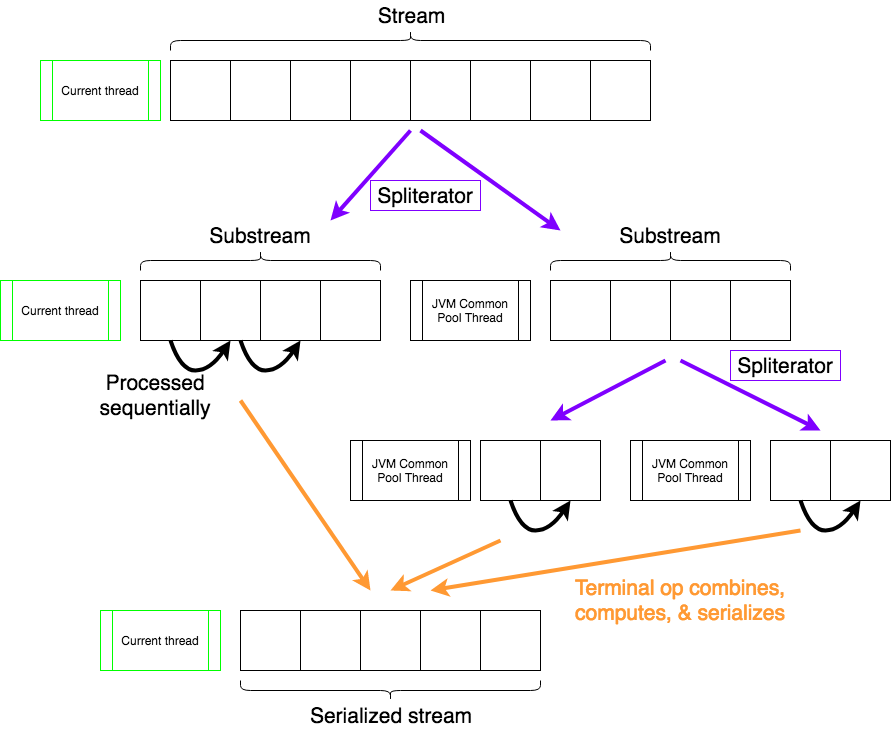
\includegraphics[width=13cm]{../images/overview.png}
\caption{Overview of a parallel stream}
\source{Ethan Williams}
\label{fig:overview}
\end{figure}

The \verb|collect()| method is the best strategy for reduction of a parallel stream because ordering of elements isn't guaranteed \autocite{ibm_streams}. The method uses a \verb|Collector| to reduce the stream, an object that defines how input elements should be added to a given data structure. This document will focus on the \verb|Collector|'s functionality and implementation, finishing with an explanation of special use cases for parallel streams.

Despite parallel streams being introduced into Java to simplify concurrency, developers can easily corrupt data and cause system bugs. All possible bugs in streams derive from developers not following standard concurrency practices such as using long-running or blocking operations in streams. Additionally, considerations have to be taken with streams specifically to avoid interference with the source and using stateful expressions.

\section{Spliterator}
The \verb|Spliterator| is the backbone of parallel streams, allowing the program to split a collection apart (illustrated in Figure \ref{fig:split}) and iterate through it \autocite{rapid7_overview}. If a class extending a \verb|Collection| does not have a \verb|spliterator()| method returning a \verb|Spliterator| object, then Java is not able to process the collection with a parallel stream at all. Figure \ref{fig:split} shows how an instance may behave when it splits itself. It is worth noting that the splitting doesn't actually break up the collection. \verb|Spliterator|s share the collection and simply keep track of what element it is currently iterating on (index) and one more than the last element it is allowed to execute with (fence).

\begin{figure}[H]
\centering
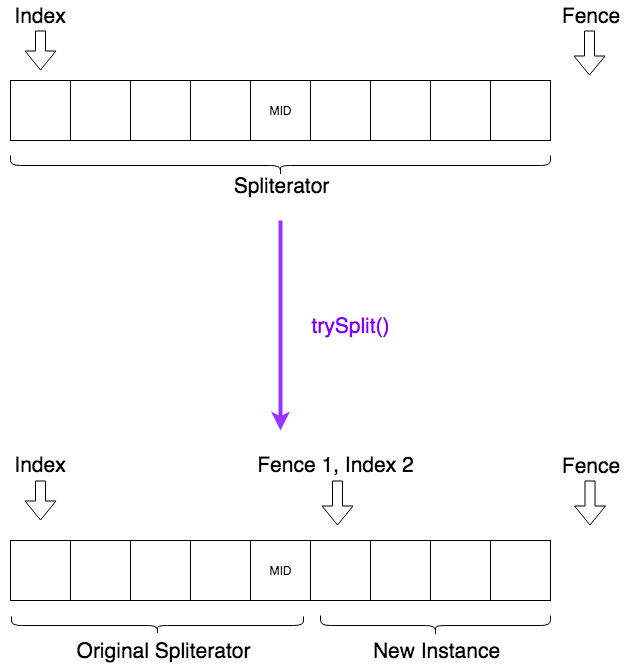
\includegraphics[width=8cm]{../images/spliterator.png}
\caption{A {\tt Spliterator} Before and after splitting}
\source{Ethan Williams}
\label{fig:split}
\end{figure}

\subsection{Implementation} 
A \verb|Spliterator| must be able to traverse and split the portion of the stream it represents. \verb|tryEachRemaining()| and \verb|tryNext()| are the two methods which dictate how traversal is handled for the collection \autocite{split_doc}. \verb|tryEachRemaining()| in Figure \ref{fig:forEachRemaining} takes a Consumer object which is the operation to be executed on each element of the collection. The example simply iterates through each element and uses it as a parameter to the \verb|accept()| method of the \verb|Consumer| object. \verb|tryNext()| in Figure \ref{fig:tryAdvance} is similar although the operation is only attempted on element at the current cursor position. If that cursor position is past the fence of the Spliterator, then the method returns false, otherwise it returns true.

\begin{figure}[H]
\centering
\begin{lstlisting}[language=Java]
public void forEachRemaining(Consumer<? super E> action) {
        for (int i = index; i < fence; ++i)  action.accept((E) list.elementData[i]);
}
\end{lstlisting}
\caption{Implementation of {\tt forEachRemaining()}}
\source{Java ArrayList, modified by Ethan Williams}
\label{fig:forEachRemaining}
\end{figure}

\begin{figure}[H]
\centering
\begin{lstlisting}[language=Java]
public boolean tryAdvance(Consumer<? super E> action) {
    if(i == fence) return false;
    index++;
    action.accept((E) list.elementData[i]);
    return true;
}
\end{lstlisting}
\caption{Implementation of {\tt tryAdvance()}}
\source{Java ArrayList, modified by Ethan Williams}
\label{fig:tryAdvance}
\end{figure}

A \verb|Spliterator|'s primary functionality is encapsulated within the \verb|trySplit()| method in Figure \ref{fig:trySplit}. This method is called when the JVM wants to break the source collection in order to start processing the stream on another thread and if implemented incorrectly can be a subtle but important error in an application \autocite{split_doc}. The example implementation simply finds the midpoint and either returns a new \verb|Spliterator| from the cursor to the midpoint and the current instance of \verb|Spliterator| now covers mid to the fence. The example \verb|trySplit()| method is the code behind the split behavior illustrated in Figure \ref{fig:split}.

\begin{figure}[H]
\centering
\begin{lstlisting}[language=Java]
public Spliterator<E> trySplit() {
    int mid = (index + fence) >>> 1;
    return (index >= mid) ? null : new Spliterator<E>(list, index, index = mid);
}
\end{lstlisting}
\caption{Implementation of {\tt trySplit()}}
\source{Java ArrayList, modified by Ethan Williams}
\label{fig:trySplit}
\end{figure}

\section{Collector}
A \verb|Collector| object defines a mutable reduction operation for a group of input elements \autocite{collector_doc}. In other words, it provides information on how to instantiate a data structure and perform several operations on it. Its functionality is encompassed in 4 methods (illustrated in Figure \ref{fig:collector}):

\begin{itemize}
\item \verb|supplier()| provides information on how to construct a new instance of the desired data structure
\item \verb|accumulator()| details how to add any given element to the data structure
\item \verb|combine()| directs how to assemble multiple instances of the data structure
\item \verb|finisher()|  simply serializes the stream, completing the reduction
\end{itemize}

\begin{figure}[H]
\centering
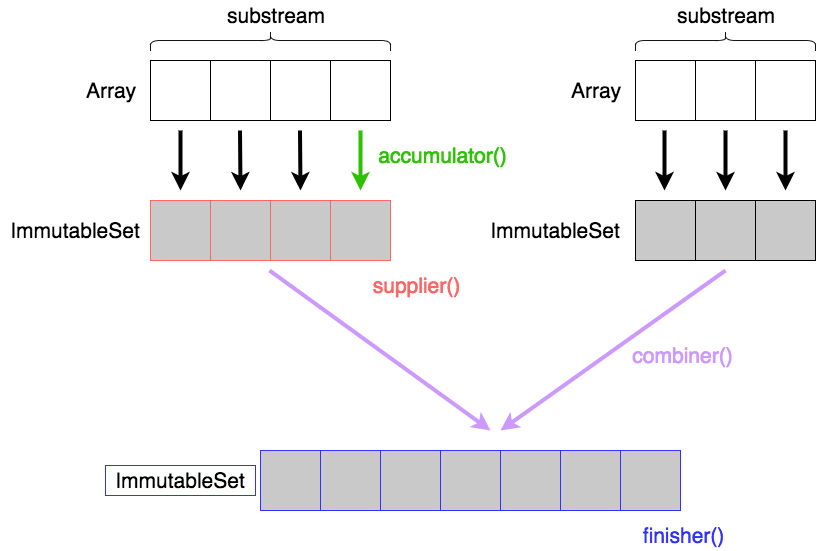
\includegraphics[width=13cm]{../images/collector.png}
\caption{How a {\tt Collector} is used}
\source{Ethan Williams}
\label{fig:collector}
\end{figure}

\verb|Collector| objects are used during a reduction operation to join substreams together in the form of the data structure defined by the instance. Java has a static class called \verb|Collectors| which provide basic reduction instances via method calls. For example \verb|Collectors.toMap()| returns a \verb|Collector| instance which reduces the stream to a \verb|Map| \autocite{collectors_doc}. 

\subsection{Implementation}

A \verb|Collector| object has four methods which comprise the majority of its functionality: \verb|supplier()|, \verb|accumulator()|, \verb|combiner()|, and \verb|finisher()| \autocite{collector_doc}. The examples below are a \verb|Collector| which will yield an \verb|ImmutableSet| when used.

The \verb|supplier()| method returns a mechanism to build an instance of a mutable data structure that will hold the elements of the stream called an \textit{accumulator} \autocite{custom_collector}, in our code example this is a builder for \verb|ImmutableSet|.

\begin{figure}[H]
\centering
\begin{lstlisting}[language=Java]
public Supplier<ImmutableSet.Builder<T>> supplier() {
    return ImmutableSet::builder;
}
\end{lstlisting}
\caption{Implementation of {\tt supplier()}}
\source{\autocite{custom_collector}}
\label{fig:supplier}
\end{figure}

The \verb|accumulator()| method takes an accumulator and an element as parameters and will return a \verb|Consumer| object which details how the element should be added to the accumulator. In the example a \verb|BiConsumer| object will add the element to the given \verb|ImmutableSet|.

\begin{figure}[H]
\centering
\begin{lstlisting}[language=Java]
public BiConsumer<ImmutableSet.Builder<T>, T> accumulator() {
    return (builder, t) -> builder.add(t);
}
\end{lstlisting}
\caption{Implementation of {\tt accumulator()}}
\source{\autocite{custom_collector}}
\label{fig:accumulator}
\end{figure}

The \verb|combiner()| method details the logic on how two accumulators should be joined together and is used to assemble all instances of the new data structure that were derived from substreams. In the code example the \verb|combiner()|'s behavior is that when two \verb|ImmutableSet|s are combined, one is simply appended to the other.

\begin{figure}[H]
\centering
\begin{lstlisting}[language=Java]
public BinaryOperator<ImmutableSet.Builder<T>> combiner() {
    return (left, right) -> {
        left.addAll(right.build());
        return left;
    };
}
\end{lstlisting}
\caption{Implementation of {\tt combiner()}}
\source{\autocite{custom_collector}}
\label{fig:combiner}
\end{figure}

Finally, the \verb|finisher()| method serializes the accumulator that is the result of combining all the substreams, completing the reduction. In the code example, this is as easy as returning the \verb|build()| method which serializes the \verb|ImmutableSet|, completing the conversion of the source.

\begin{figure}[H]
\centering
\begin{lstlisting}[language=Java]
public Function<ImmutableSet.Builder<T>, ImmutableSet<T>> finisher() {
    return ImmutableSet.Builder::build;
}
\end{lstlisting}
\caption{Implementation of {\tt finisher()}}
\source{\autocite{custom_collector}}
\label{fig:finisher}
\end{figure}

\subsection{Special Uses for Parallelism}
Although the \verb|collect()| method can be used on both serial and parallel streams, Java also includes special \verb|Collector| instances for parallel performance. For example, Figure \ref{fig:employee_collection} shows two parallel streams where the first one utilizes the \verb|groupingBy()| method and the other one uses \verb|groupingByConcurrent()|. Although Java's official documentation says the second should be more performant \autocite{parallelism_doc}, in my benchmarks that I ran I got a significant slowdown, .736 ms/op vs 2.533 ms/op \autocite{benchmark_software}. Additional research as to why this is the case yielded no results and as such the author suggests every developer should benchmark these operations themselves to validate performance.

\begin{figure}[H]
\centering
\begin{lstlisting}[language=Java]
// Example 1
ConcurrentHashMap<Department, List<Employee>> byDept
    = employees.stream()
               .parallel()
               .collect(Collectors
                  .groupingBy(Employee::getDepartment)
                );
                
// Example 2
Map<Department, List<Employee>> byDept
    = employees.stream()
               .parallel()
               .collect(Collectors
                  .groupingByConcurrent(Employee::getDepartment)
                );
\end{lstlisting}
\caption{Reduction of employees into map by a {\tt Collector}}
\source{Ethan Williams}
\label{fig:employee_collection}
\end{figure}

\section{Practical Considerations when Using Parallel Streams}
Parallel streams were introduced to make implementing parallelism in a Java application easier, but with this ease comes common pitfalls that arise from the abstraction. For example, a common mistake is using long-running or blocking operations in a stream which is a bad concurrency practice to begin with. Additionally, many developers aren't familiar with stream-specific concurrency practices which can lead to bugs. These are known as  interference and use of stateful expressions and are extremely difficult to debug.

\subsection{Long-Running/Blocking Operations}
Using long-running or blocking operations in a stream will degrade performance drastically, a result of how streams implement threading. The JVM begins by processing on the calling thread and as more subtasks are broken off, the JVM gets threads from \verb|ForkJoinPool.common()|, which is a thread pool used in the background of the whole application \autocite{dzone_dangers}. 

With the JVM's use of a common thread pool, a long-running operation in a parallel stream as shown in the first example of Figure \ref{fig:network_op} will degrade performance drastically. Benchmarking puts both of these operations at the same runtime, but the parallel version can degrade performance of other parallel streams that are being processed in the application \autocite{benchmark_software}.

In a situation where several streams are all attempting to process in parallel, each stream's performance will suffer even if it should have no problem. Java does allow a custom \verb|ThreadPool| like in example 2 of Figure \ref{fig:network_op} which can help by using threads created outside the common pool \autocite{dzone_fjp}. Unfortunately, since the issue described above results from a bad concurrency practice, more threads won't provide any significant performance enhancement.

\begin{figure}[H]
\centering
\begin{lstlisting}[language=Java]
// Example 1
Optional<String> result = collection.stream().parallel().map((base) -> longOperation(argument)).findAny();

// Example 2
ForkJoinPool customPool = new ForkJoinPool(4);
Optional<String> result = customPool.submit(() -> collection.stream().parallel().map((arg) -> longOperation(arg)).findAny()).get();
\end{lstlisting}
\caption{Reduction of employees into map by a {\tt Collector}}
\source{Ethan Williams}
\label{fig:network_op}
\end{figure}

\subsection{Interference}
Since streams don't contain any of the elements of the collection, instead iterating via each \verb|Spliterator|'s index, adding to the collection can cause problems and is called \textit{interference}. Figure \ref{fig:interference} shows why this will throw a \verb|ConcurrentModificationException| \autocite{parallelism_doc}; to start, the \verb|Spliterator| starts processing elements until the index is 3. A new item is added to the beginning of the collection and now the index suggests we re-process that element while never touching the newly added element. Writing interfering code dangerous because is easy to write and Figure \ref{fig:interference} shows an extremely simple example where each element is inserted into the collection again.

\begin{figure}[H]
\centering
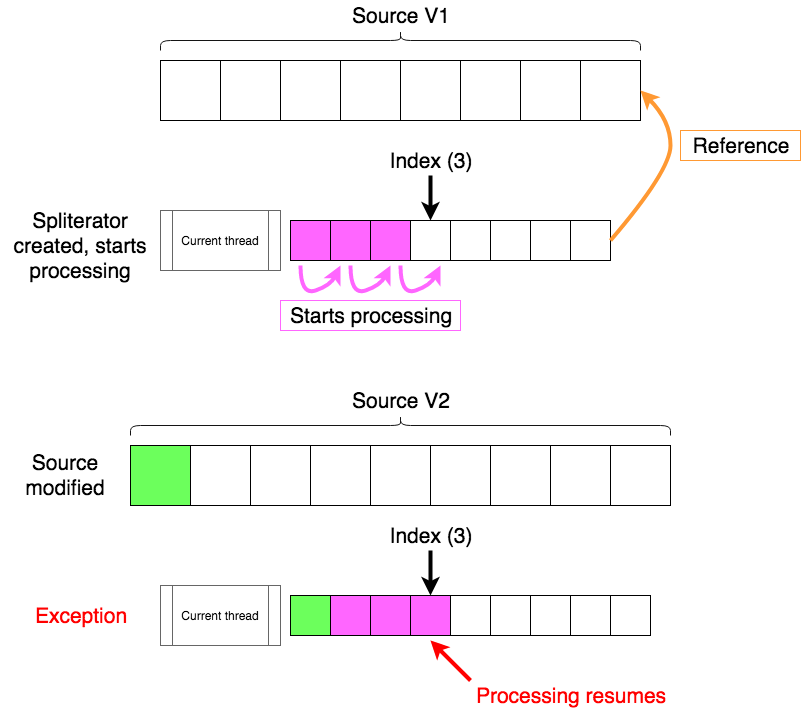
\includegraphics[width=13cm]{../images/interference.png}
\caption{Why interference is a problem}
\source{Ethan Williams}
\label{fig:interference_pic}
\end{figure}

\begin{figure}[H]
\centering
\begin{lstlisting}[language=Java]
collection.stream().parallel().map((x) -> collection.add(x)).toArray();
\end{lstlisting}
\caption{A stream which causes interference and will throw an error}
\source{Ethan Williams}
\label{fig:interference}
\end{figure}

\subsection{Stateful Expressions} \label{stateful_expressions}
The third practice which will cause errors in a stream  is using stateful expressions, operations that depend on the ordering of the elements \autocite{expression_state}. The code in Figure \ref{fig:stateful} shows an example of a stateful operation while attempting to add elements to \verb|parallelStorage| and print them. Although the \verb|forEachOrdered()| method is just fine and will print in the expected order, \verb|parallelStorage| will have a different ordering every time the stream is executed. The addition is stateful, meaning it depends on ordering and in parallel streams ordering can't be guaranteed in intermediate operations \autocite{parallelism_doc}.

\begin{figure}[H]
\centering
\begin{lstlisting}[language=Java]
List<String> parallelStorage = Collections.synchronizedList(new ArrayList<>());
collection.stream().parallel().map(x -> parallelSotrage.add(x)).forEachOrdered(x -> System.out.println(x));
\end{lstlisting}
\caption{A stream which causes interference and will throw an error}
\source{Ethan Williams}
\label{fig:stateful}
\end{figure}
 
\printbibliography[heading=bibintoc]

\end{document}